\documentclass[10pt]{article}

% COLM 2025 style (mirrors NeurIPS/ICLR layout)
\usepackage[margin=1in,top=1.25in,bottom=1.25in]{geometry}
\usepackage{times}
\usepackage{microtype}
\usepackage{graphicx}
\usepackage{booktabs}
\usepackage{amsmath}
\usepackage{amssymb}
\usepackage{natbib}
\usepackage{hyperref}
\usepackage{xcolor}
\usepackage{float}
\usepackage{subcaption}
\usepackage{array}
\usepackage{multirow}
\usepackage{tabularx}
\usepackage{enumitem}
\usepackage{parskip}

\hypersetup{
  colorlinks=true,
  linkcolor=blue!60!black,
  citecolor=blue!60!black,
  urlcolor=blue!60!black,
}

% Title formatting
\usepackage{titlesec}
\titleformat{\section}{\large\bfseries}{\thesection}{1em}{}
\titleformat{\subsection}{\normalsize\bfseries}{\thesubsection}{1em}{}
\titleformat{\subsubsection}{\normalsize\itshape}{\thesubsubsection}{1em}{}

\setlength{\parskip}{4pt}
\setlength{\parindent}{0pt}

% Abstract environment
\renewenvironment{abstract}{%
  \begin{center}
    \textbf{Abstract}
  \end{center}
  \begin{quote}
}{%
  \end{quote}
  \vspace{0.5em}
}

\title{\textbf{Evaluating Cross-Lingual Performance and Implicit Translation\\
in Large Language Models}}

\author{
  Kai Lee \quad Justin Tarquino \\
  University of Chicago \\
  \texttt{\{kailee, jtarquino\}@uchicago.edu}
}

\date{}

\begin{document}
\maketitle

\begin{abstract}
Large language models (LLMs) are trained predominantly on English data yet deployed in
multilingual contexts, raising open questions about how well they generalize across
languages and whether they rely on implicit translation mechanisms when processing
non-English inputs. We study these questions through a two-pronged framework: black-box
accuracy evaluation and white-box mechanistic probing via logit lens and
Representational Similarity Analysis (RSA). We construct a 180-question benchmark
spanning three languages---English, Spanish, and Basque---and three task categories
(math, factual, reasoning), and evaluate two 7B-parameter instruction-tuned models:
Mistral-7B-Instruct-v0.2 and Qwen2-7B-Instruct. Mistral achieves 68\% overall
English accuracy but collapses to 8\% on Basque (0\% factual); Qwen2 is significantly
more robust at 37\% Basque overall. Logit lens reveals that math answers are identified
at shallow layers regardless of language, while Basque factual representations become
structurally random by the final layer. RSA across all 32 layers provides evidence for
implicit translation in reasoning tasks: English-Spanish representational similarity
peaks in mid-layers (Spearman \(r = 0.81\) at layer 8) before declining at the output
stage, consistent with a shared cross-lingual computation resolved in a
language-specific way. Together, our results show that cross-lingual performance
disparities are not merely behavioral but are reflected deep in the residual stream,
and that the degree of cross-lingual representational alignment differs substantially
by task category and language pair.
\end{abstract}

%% ============================================================
\section{Introduction}
%% ============================================================

LLMs are deployed multilingually but trained heavily on English \citep{ahuja2023mega}; accuracy often drops for non-English inputs, yet \emph{why} and \emph{how} processing fails across layers remains unclear. A central hypothesis is \emph{implicit internal translation}: non-English input is mapped to an internal representation before an answer is computed \citep{wendler2024llamas}. For low-resource languages like Basque, models may tokenize but fail to process meaningfully.

Our work investigates two complementary questions:
\begin{enumerate}[leftmargin=*,itemsep=0pt]
  \item \textbf{Behavioral:} How do accuracy and generation quality vary across English,
  Spanish, and Basque, and across math, factual, and reasoning task categories?
  \item \textbf{Mechanistic:} Do the residual stream representations of semantically
  equivalent questions across languages share relational structure (RSA), and does
  cross-lingual representational similarity arise and decay at predictable layers
  (logit lens)?
\end{enumerate}

We build a 180-question aligned benchmark (EN/ES/Basque), run two 7B models with full hidden-state extraction, and combine black-box accuracy with logit lens and RSA. Contributions: (1) a lightweight multilingual benchmark with LLM-as-judge evaluation; (2) logit lens showing math language-agnostic at shallow layers and Basque factual failing to converge; (3) RSA evidence for implicit translation (EN--ES reasoning peaks mid-layer then declines); (4) cross-model comparison showing Mistral vs.\ Qwen2 use different multilingual representational strategies.

%% ============================================================
\section{Related Work}
%% ============================================================

\paragraph{Multilingual LLM benchmarks.}
Benchmarks remain English-centric \citep{hendrycks2020measuring}; INCLUDE \citep{include2024} and other work add many languages but focus on accuracy, not internal representations. We pair a small benchmark with white-box probing for mechanistic interpretation.

\paragraph{Cross-lingual generalization \& implicit translation.}
\citet{ahuja2023mega} find consistent low-resource degradation; \citet{wendler2024llamas} argue for English-centric latent spaces. We analyze alignment at every layer and link it to task-specific accuracy; RSA shows mid-layer peaks for reasoning consistent with implicit translation.

\paragraph{Logit lens \& RSA.}
The logit lens \citep{nostalgebraist2020logitlens} decodes layer-wise ``predictions''; RSA compares representational geometry. We apply both multilingually: GT rank and confidence by layer, and layer-wise RSA for relational structure across languages.

%% ============================================================
\section{Experimental Design}
\label{sec:methods}
%% ============================================================

\subsection{Benchmark Construction}

We constructed a benchmark of 180 questions organized as aligned triplets: each
question appears in English, Spanish, and Basque, sharing the same ground-truth
answer. Questions are split into three categories (20 questions each per language):

\begin{itemize}[leftmargin=*,itemsep=1pt]
  \item \textbf{Math:} Arithmetic, algebra, and geometry problems. Answers are
  numerals or short symbolic expressions, minimizing lexical variation across languages.
  \item \textbf{Factual:} World knowledge questions covering science, geography, and
  history. Requires retrieval of facts likely represented unevenly across languages
  in the training corpus.
  \item \textbf{Reasoning:} Logic puzzles, lateral thinking, and trick questions.
  Requires structural inference; we hypothesize reasoning structure may be shared
  cross-lingually in intermediate layers.
\end{itemize}

Table~\ref{tab:benchmark_examples} shows one aligned triplet per task: the same item in English, Spanish, and Basque with shared ground-truth answers.

\begin{table}[H]
\centering
\caption{Example benchmark questions by language and task (aligned triplets share the same ground-truth answer).}
\label{tab:benchmark_examples}
\small
\begin{tabular}{@{}l p{3.6cm} p{3.6cm} p{3.8cm} @{}}
\toprule
\textbf{Language} & \textbf{Math} & \textbf{Factual} & \textbf{Reasoning} \\
\midrule
English
  & Question: What is the sum of 15 and 27? Answer: 42
  & Question: What is the capital of France? Answer: Paris
  & Question: A is taller than B, and B is taller than C. Who is the shortest? Answer: C \\
\addlinespace
Spanish
  & Question: ¿Cuál es la suma de 15 y 27? Answer: 42
  & Question: ¿Cuál es la capital de Francia? Answer: París
  & Question: A es más alto que B, y B es más alto que C. ¿Quién es el más bajo? Answer: C \\
\addlinespace
Basque
  & Question: 15 eta 27 ren batura zer da? Answer: 42
  & Question: Frantziako hiriburua zein da? Answer: Paris
  & Question: A, B baino altuagoa da, eta B, C baino altuagoa. Nor da baxuena? Answer: C \\
\bottomrule
\end{tabular}
\end{table}

We selected a three-language gradient to span high-resource (English), medium-resource
(Spanish, Indo-European), and low-resource (Basque, language isolate with no close
relatives and minimal training data representation). Original questions were written
in English and translated to Spanish and Basque via GPT-4, with manual verification
to ensure semantic equivalence and avoid translation artifacts.

\subsection{Models}

We evaluate two 7B-parameter instruction-tuned models:
\begin{itemize}[leftmargin=*,itemsep=1pt]
  \item \textbf{Mistral-7B-Instruct-v0.2:} 32 transformer layers, $d_\text{model}=4096$,
  vocabulary size 32,000. We use the \texttt{[INST]\allowbreak ...\allowbreak [/INST]} prompt format.
  \item \textbf{Qwen2-7B-Instruct:} 28 transformer layers, $d_\text{model}=3584$,
  vocabulary size 152,064 (a significantly larger multilingual vocabulary). We use
  the Qwen2 chat template.
\end{itemize}

Both models were run on A100 GPUs via Modal in \texttt{float16} with greedy decoding
and \texttt{max\_new\_tokens=50}. We use a single unified model for both black-box
accuracy and all white-box probing, avoiding the cross-model confound present in
our early-phase experiments where we used GPT-3.5-turbo and Gemini for inference but
BLOOM-560M for probing.

\subsection{Black-Box, Logit Lens, and RSA}
\label{sec:blackbox}

\textbf{Black-box:} We record free-form generations for all 180 questions and score with an LLM-as-judge (GPT-4o-mini / Grok-3-mini, binary YES/NO); results cached for reproducibility.

\textbf{Logit lens:} At each layer $\ell$, we project last-token $\mathbf{h}^{(\ell)}$ through final LayerNorm and LM head to get $p^{(\ell)} = \text{softmax}(W_{\text{lm}} \cdot \text{LayerNorm}(\mathbf{h}^{(\ell)}))$. We record GT rank (rank of first ground-truth token in $p^{(\ell)}$) and top-1 confidence $\max_t p^{(\ell)}_t$.

\textbf{RSA:} For each (language, category) we extract last-token residual vectors at every layer and build $20{\times}20$ RDMs: $\text{RDM}^{(\ell)}_{ij} = 1 - \cos(\mathbf{h}^{(\ell)}_i, \mathbf{h}^{(\ell)}_j)$. We compute Spearman $r$ between RDMs for each language pair at each layer; high $r$ means similar relational structure across languages.

%% ============================================================
\section{Results}
%% ============================================================

\subsection{Black-Box Accuracy}
\label{sec:results_accuracy}

Table~\ref{tab:accuracy} and Figure~\ref{fig:accuracy_heatmap} summarize black-box
accuracy across all language-category combinations for both models.

\begin{table}[H]
\centering
\caption{Black-box accuracy (\%) by language, category, and model. \textbf{Bold}
indicates best result per cell. Qwen2-7B is substantially more robust on Basque across
all categories.}
\label{tab:accuracy}
\begin{tabular}{llcc}
\toprule
\textbf{Language} & \textbf{Category} & \textbf{Mistral-7B} & \textbf{Qwen2-7B} \\
\midrule
\multirow{4}{*}{English}
  & Math      & 45 & \textbf{55} \\
  & Factual   & \textbf{100} & \textbf{100} \\
  & Reasoning & \textbf{60} & \textbf{60} \\
  & \textit{Overall} & 68 & \textbf{72} \\
\midrule
\multirow{4}{*}{Spanish}
  & Math      & 50 & \textbf{70} \\
  & Factual   & \textbf{100} & 95 \\
  & Reasoning & 35 & \textbf{65} \\
  & \textit{Overall} & 62 & \textbf{77} \\
\midrule
\multirow{4}{*}{Basque}
  & Math      & 20 & \textbf{65} \\
  & Factual   & 0  & \textbf{30} \\
  & Reasoning & 5  & \textbf{15} \\
  & \textit{Overall} & 8  & \textbf{37} \\
\bottomrule
\end{tabular}
\end{table}

\begin{figure}[H]
\centering
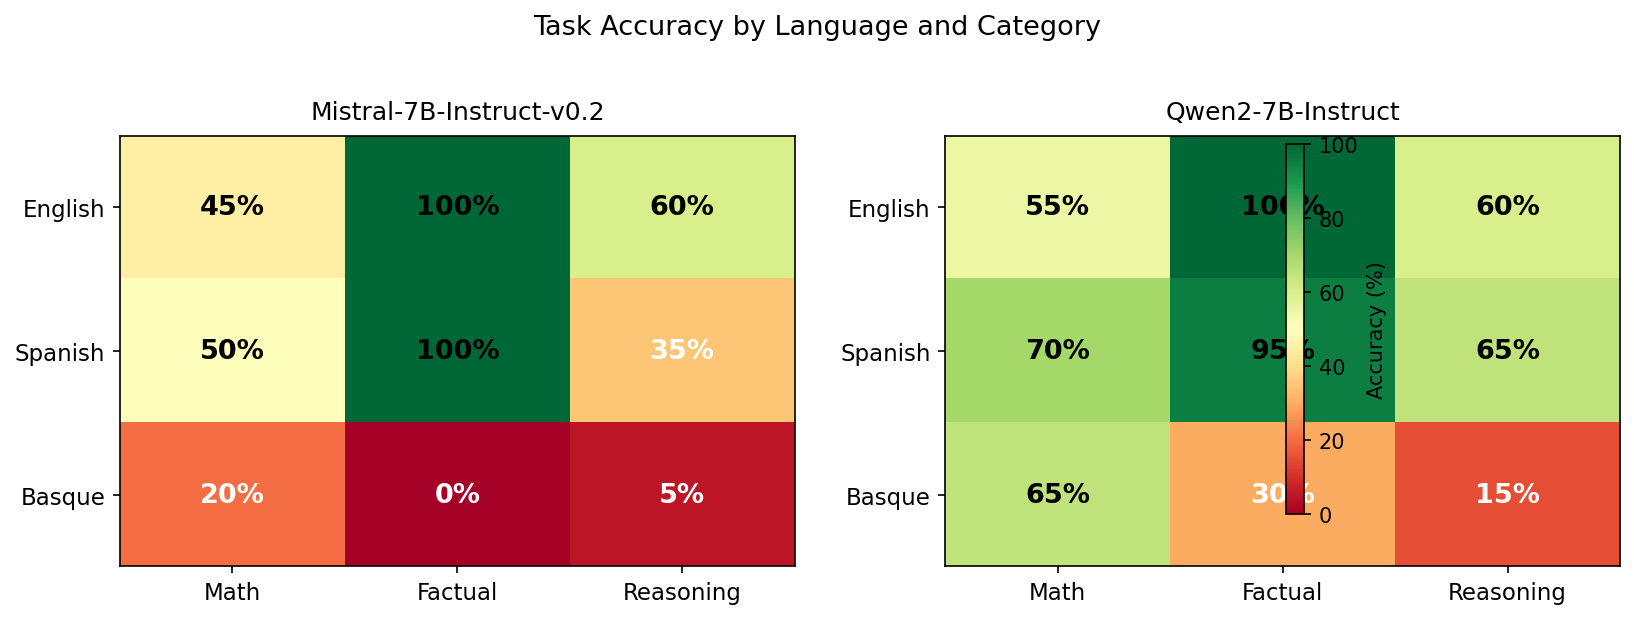
\includegraphics[width=\linewidth]{figures/fig1_accuracy_heatmap.png}
\caption{Accuracy by language and category (Mistral left, Qwen2 right). Qwen2 much stronger on Basque; both 100\% English factual.}
\label{fig:accuracy_heatmap}
\end{figure}

\subsection{Logit Lens: Layer-by-Layer Prediction Trajectories}
\label{sec:results_logitlens}

\begin{table}[H]
\centering
\caption{Logit lens summary for Mistral-7B-Instruct-v0.2: mean ground-truth rank (lower
is better) and mean top-1 confidence at layers 1 and 32.}
\label{tab:logitlens}
\begin{tabular}{llcccc}
\toprule
& & \multicolumn{2}{c}{\textbf{GT Rank}} & \multicolumn{2}{c}{\textbf{Top-1 Conf.}} \\
\cmidrule(lr){3-4}\cmidrule(lr){5-6}
\textbf{Language} & \textbf{Category} & \textbf{L1} & \textbf{L32} & \textbf{L1} & \textbf{L32} \\
\midrule
\multirow{3}{*}{English}
  & Math      & 1,160 & 261   & 0.001 & \textbf{0.942} \\
  & Factual   & 12,041 & \textbf{26} & 0.001 & \textbf{0.978} \\
  & Reasoning & 5,652  & 186  & 0.001 & 0.870 \\
\midrule
\multirow{3}{*}{Spanish}
  & Math      & 1,143  & 452  & 0.001 & 0.810 \\
  & Factual   & 14,912 & 219  & 0.001 & 0.768 \\
  & Reasoning & 11,241 & 309  & 0.001 & 0.688 \\
\midrule
\multirow{3}{*}{Basque}
  & Math      & \textbf{339} & \textbf{62} & 0.001 & 0.703 \\
  & Factual   & 10,434 & 2,440 & 0.001 & 0.848 \\
  & Reasoning & 5,690  & 108  & 0.001 & 0.539 \\
\bottomrule
\end{tabular}
\end{table}

\begin{figure}[H]
\centering
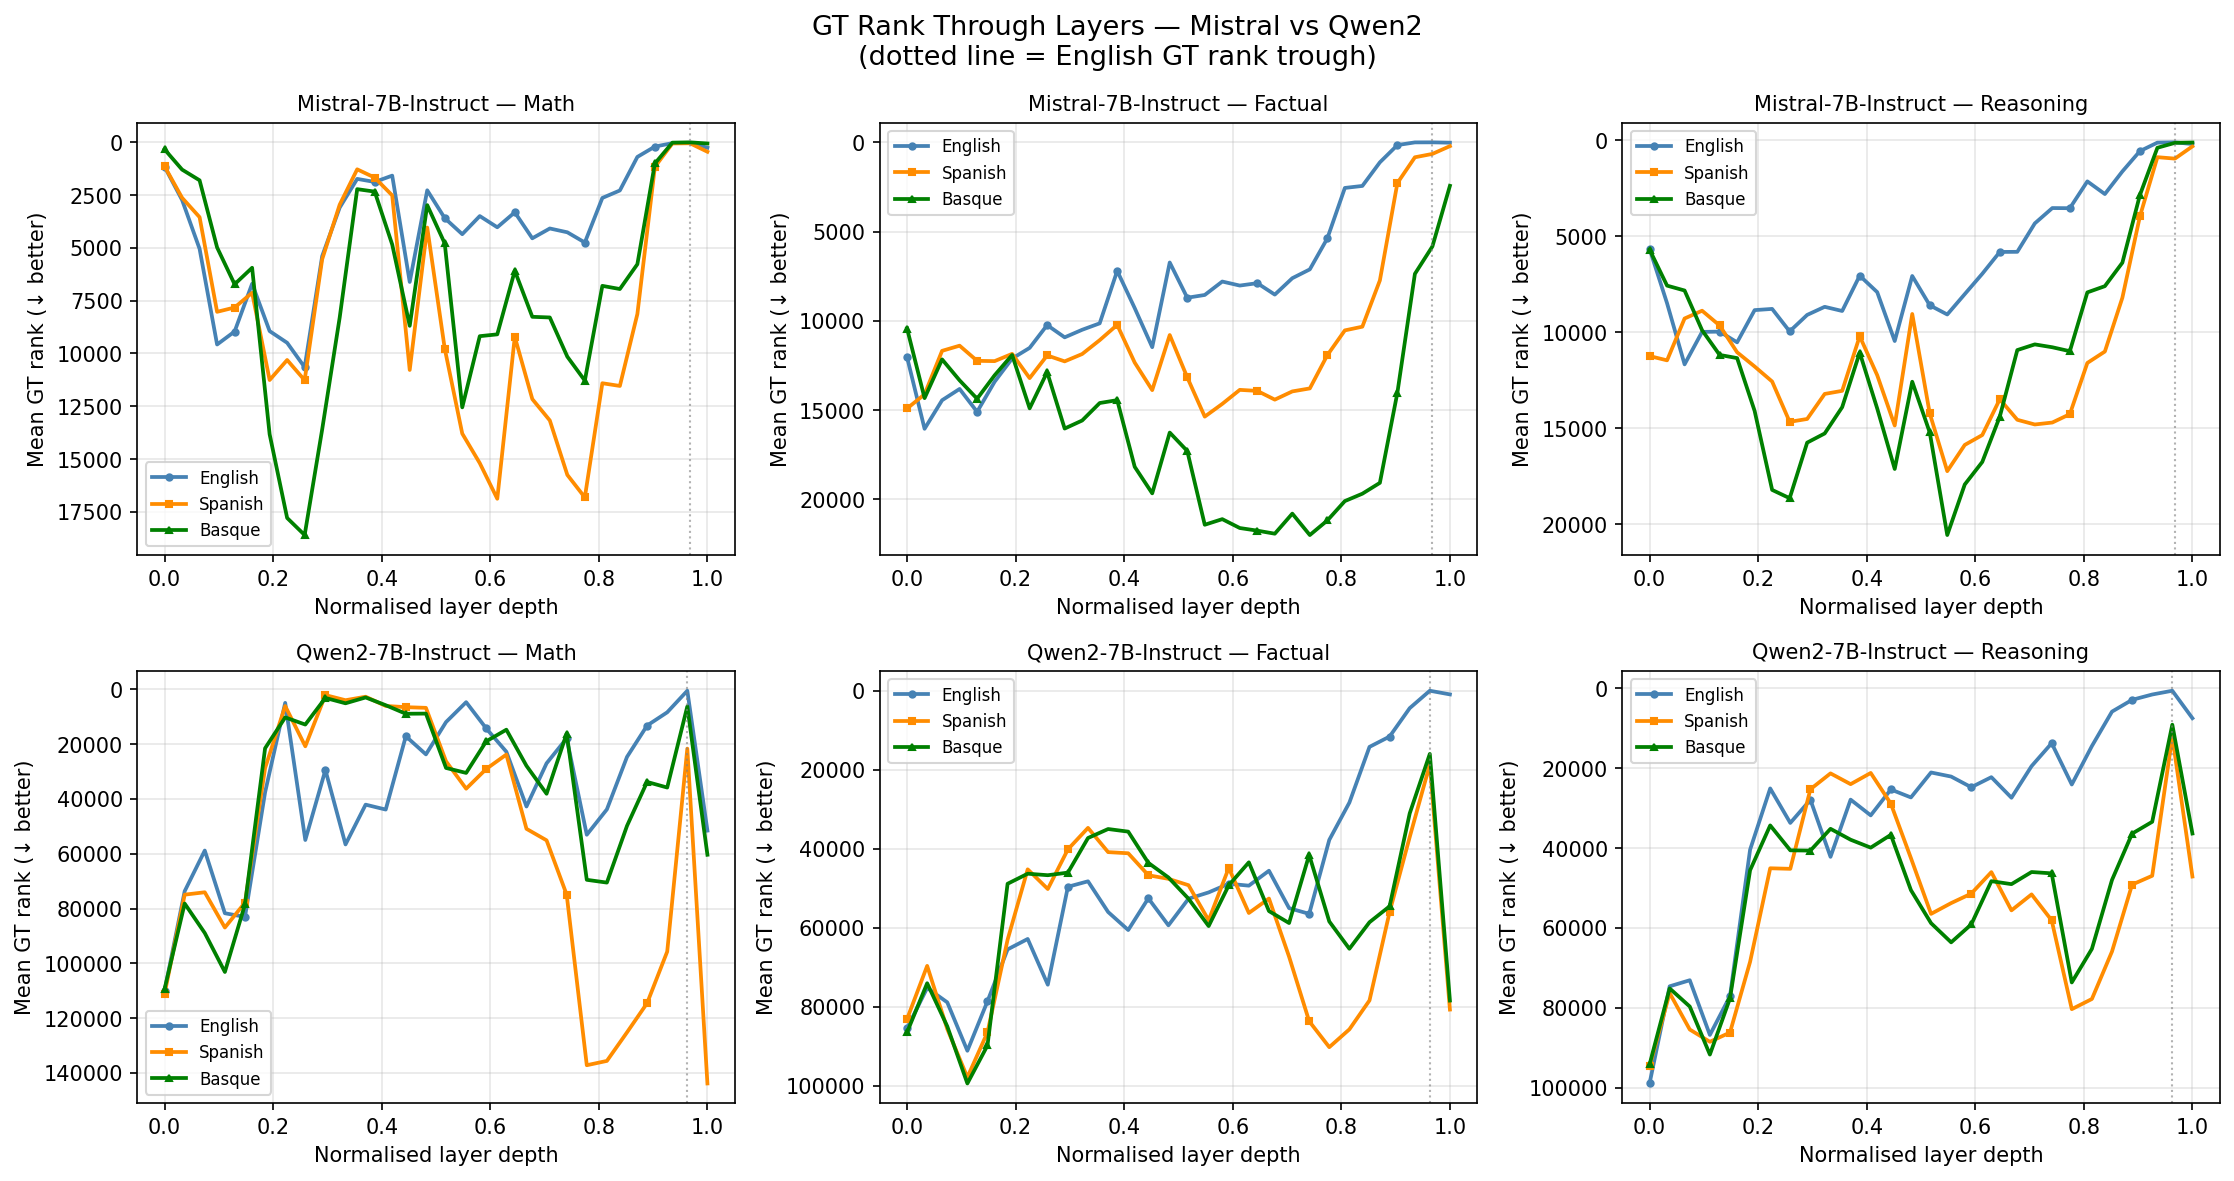
\includegraphics[width=\linewidth]{figures/fig2_gt_rank_both_models.png}
\caption{Mean GT rank vs.\ normalized layer (Mistral top, Qwen2 bottom). Basque factual stays elevated in Mistral; Qwen2's larger vocab yields higher absolute ranks.}
\label{fig:gt_rank}
\end{figure}

\begin{figure}[H]
\centering
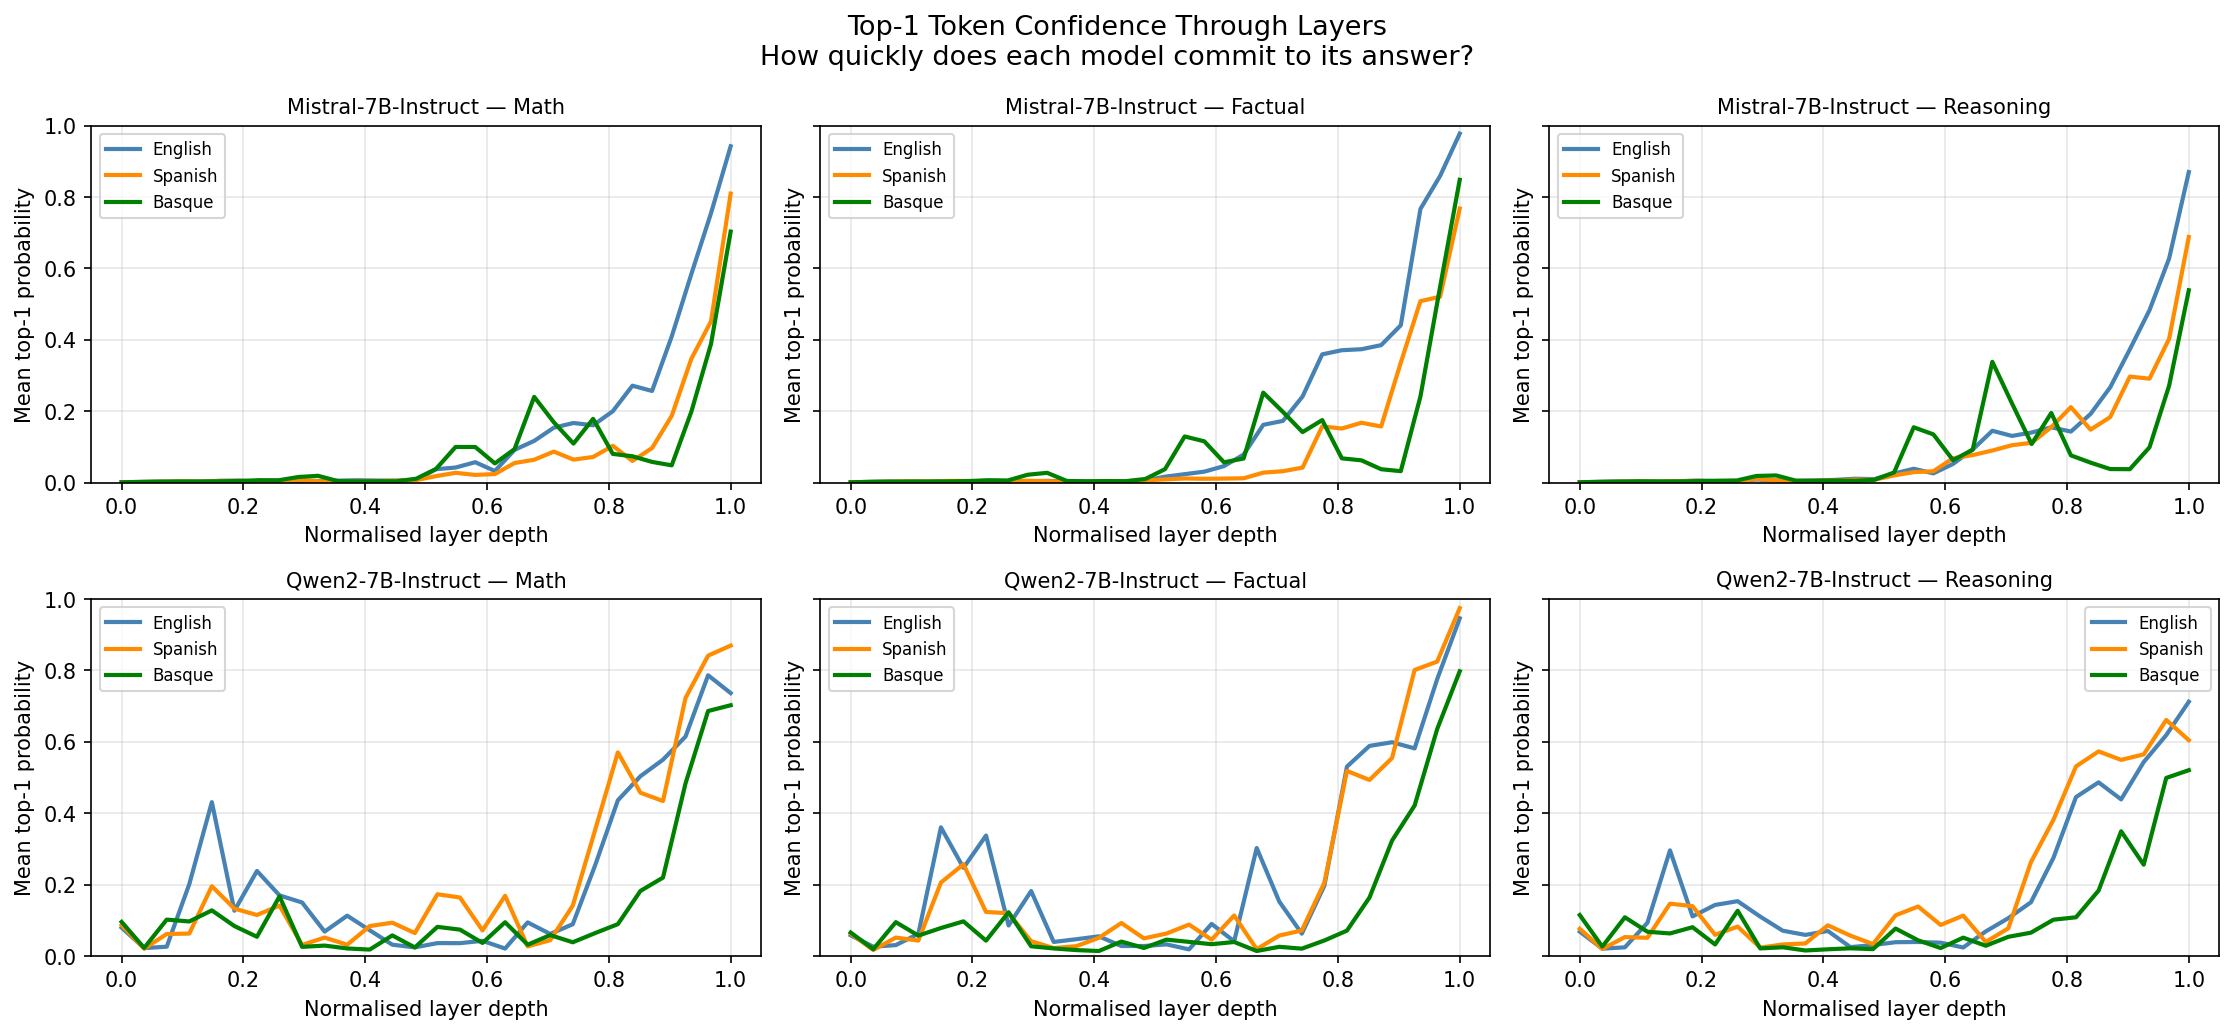
\includegraphics[width=\linewidth]{figures/fig3_confidence_both_models.png}
\caption{Mean top-1 confidence vs.\ layer. Basque reasoning has lowest final confidence (Mistral), consistent with 5\% accuracy.}
\label{fig:confidence}
\end{figure}

\subsection{RSA: Cross-Lingual Representational Alignment}
\label{sec:results_rsa}

\begin{table}[H]
\centering
\caption{RSA Spearman $r$ between language-pair RDMs at selected layers, for Mistral-7B.
Bold: highest correlation per row. Underline: negative (anti-correlated) values.}
\label{tab:rsa}
\begin{tabular}{llccccc}
\toprule
\textbf{Category} & \textbf{Pair} & \textbf{L1} & \textbf{L8} & \textbf{L16} & \textbf{L24} & \textbf{L32} \\
\midrule
\multirow{3}{*}{Math}
  & EN--ES & \textbf{0.906} & 0.871 & 0.834 & 0.858 & 0.785 \\
  & EN--EU & \textbf{0.807} & 0.683 & 0.299 & 0.352 & 0.389 \\
  & ES--EU & \textbf{0.846} & 0.630 & 0.496 & 0.465 & 0.273 \\
\midrule
\multirow{3}{*}{Factual}
  & EN--ES & 0.718 & \textbf{0.840} & 0.704 & 0.795 & 0.782 \\
  & EN--EU & 0.508 & 0.406 & \underline{$-$0.032} & 0.142 & \underline{$-$0.049} \\
  & ES--EU & 0.694 & 0.384 & 0.056 & 0.166 & 0.013 \\
\midrule
\multirow{3}{*}{Reasoning}
  & EN--ES & 0.394 & \textbf{0.810} & 0.706 & 0.739 & 0.558 \\
  & EN--EU & 0.303 & \underline{$-$0.097} & 0.088 & 0.023 & 0.018 \\
  & ES--EU & 0.584 & \underline{$-$0.035} & 0.104 & 0.022 & \underline{$-$0.080} \\
\bottomrule
\end{tabular}
\end{table}

\begin{figure}[H]
\centering
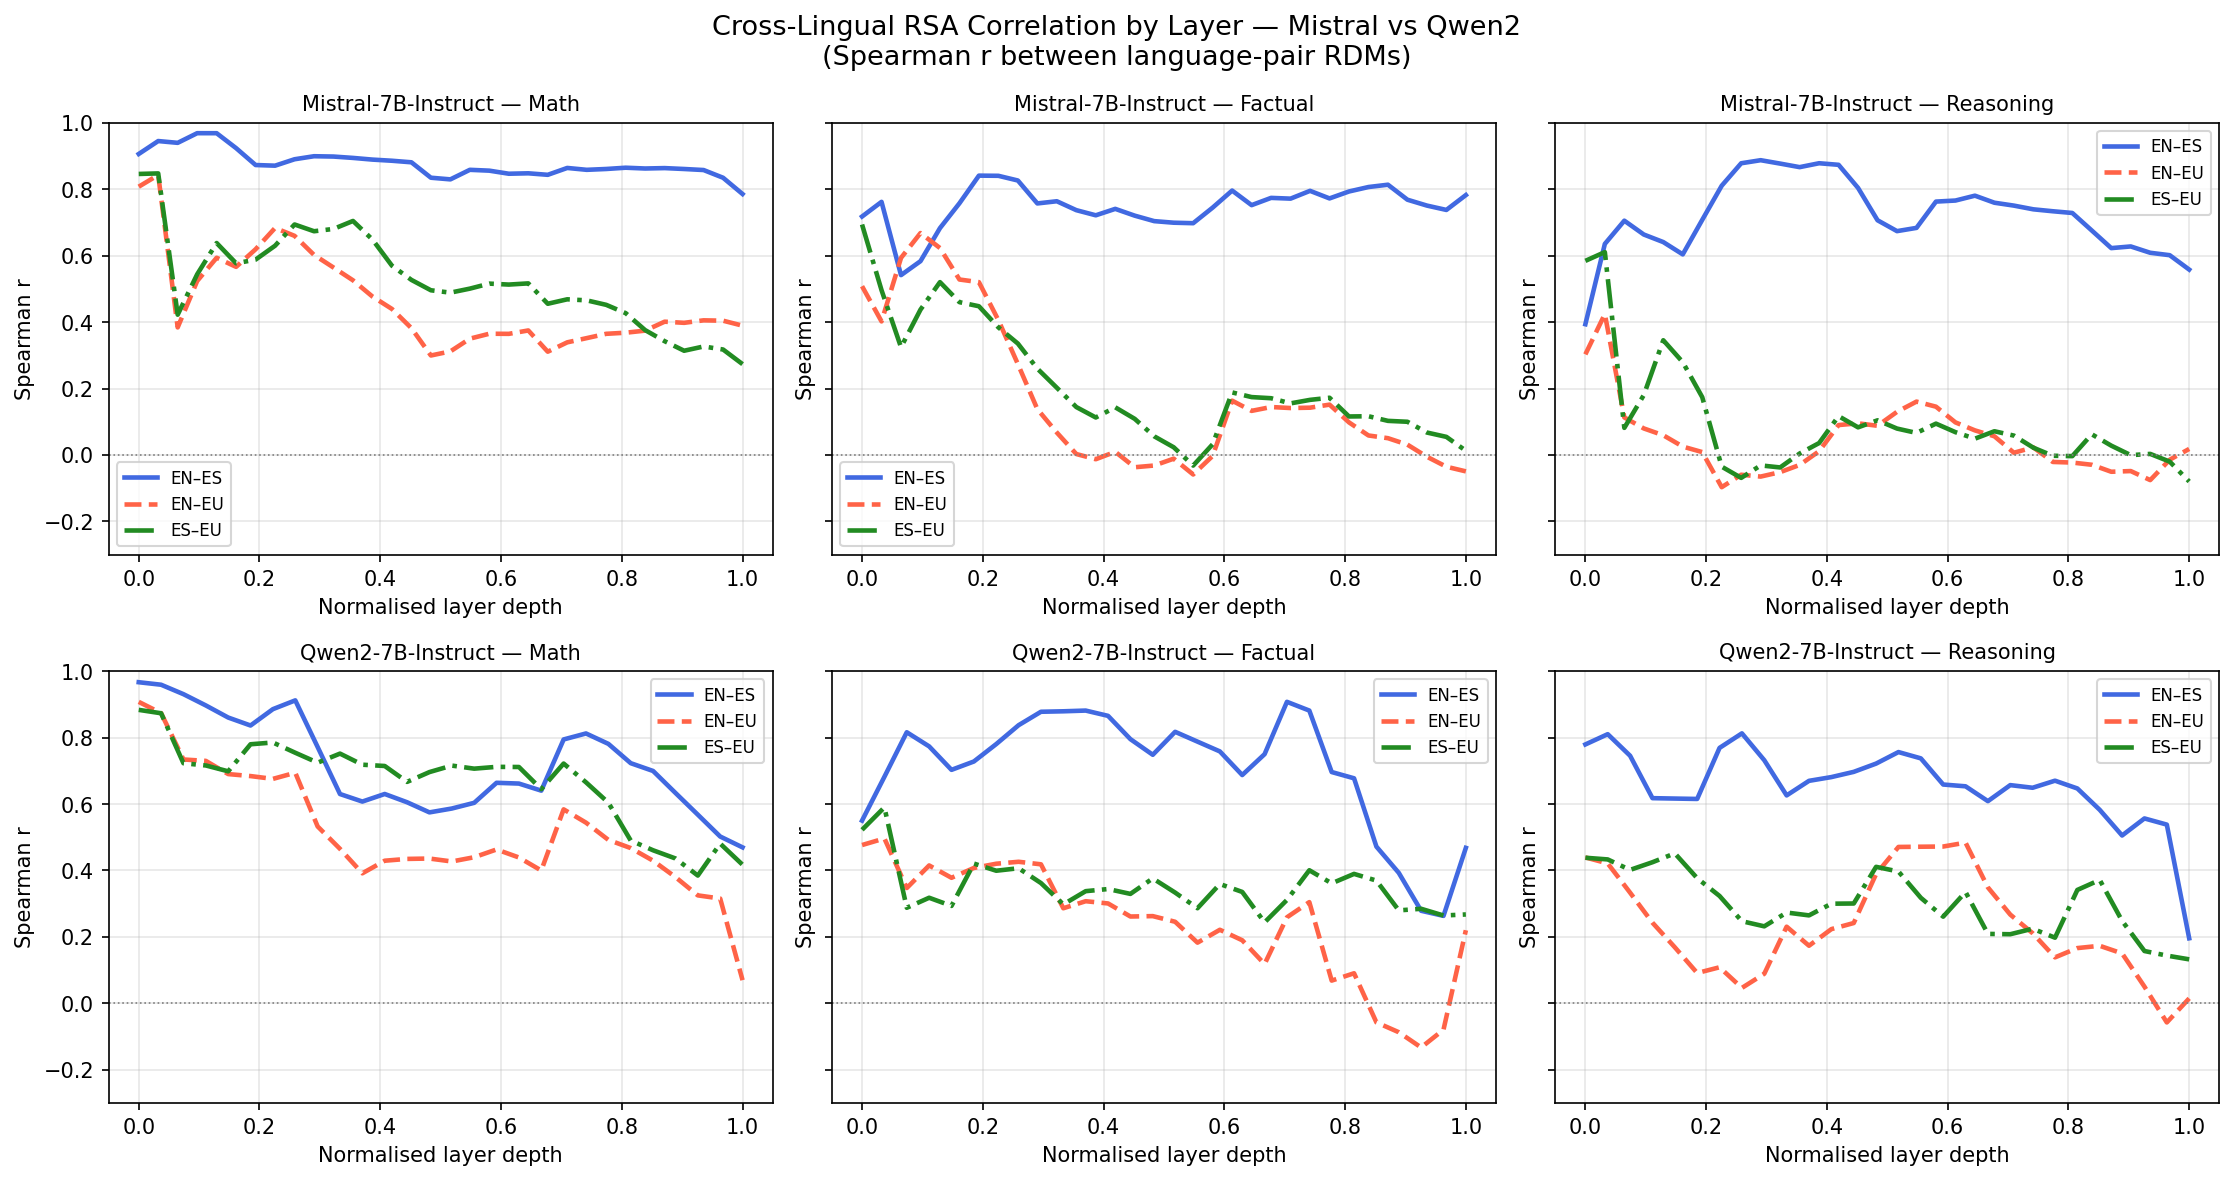
\includegraphics[width=\linewidth]{figures/fig4_rsa_both_models.png}
\caption{RSA $r$ by layer (Mistral top, Qwen2 bottom). EN--ES reasoning mid-layer peak visible in Mistral; Qwen2 has lower RSA despite higher Basque accuracy.}
\label{fig:rsa_curves}
\end{figure}

\begin{figure}[H]
\centering
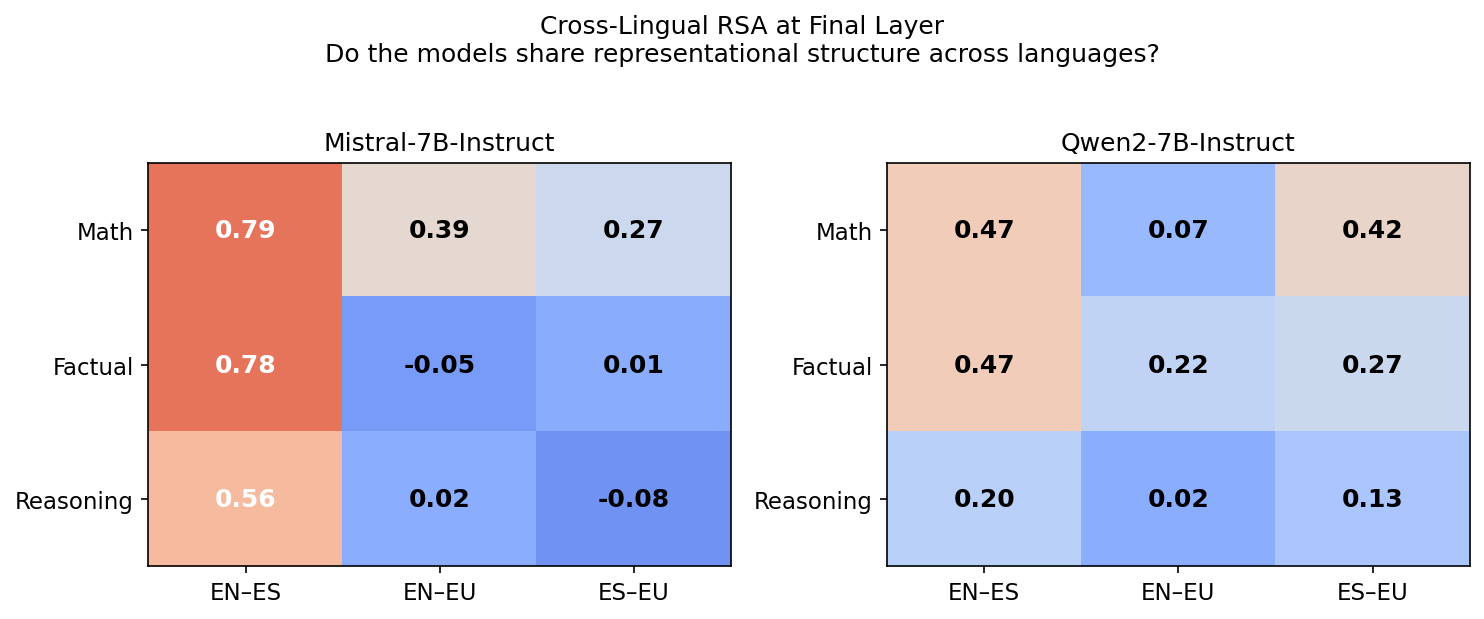
\includegraphics[width=\linewidth]{figures/fig5_rsa_final_layer_heatmap.png}
\caption{Final-layer RSA $r$ (Mistral left, Qwen2 right). EN--EU factual near zero/negative; EN--ES math highest.}
\label{fig:rsa_heatmap}
\end{figure}

\subsection{Cross-Model Comparison}
\label{sec:results_cross_model}

\begin{table}[H]
\centering
\caption{RSA Spearman $r$ at the final layer, compared between Mistral-7B and
Qwen2-7B. Bold indicates the model with higher RSA per cell. Qwen2 achieves better
Basque accuracy but shows \emph{lower} EN--ES RSA, suggesting different internal
multilingual representations.}
\label{tab:rsa_comparison}
\begin{tabular}{llccc}
\toprule
\textbf{Category} & \textbf{Pair} & \textbf{Mistral} & \textbf{Qwen2} & \textbf{$\Delta$} \\
\midrule
\multirow{3}{*}{Math}
  & EN--ES & \textbf{0.785} & 0.470 & $-$0.316 \\
  & EN--EU & \textbf{0.389} & 0.070 & $-$0.319 \\
  & ES--EU & 0.273 & \textbf{0.417} & $+$0.144 \\
\midrule
\multirow{3}{*}{Factual}
  & EN--ES & \textbf{0.782} & 0.468 & $-$0.314 \\
  & EN--EU & $-$0.049 & \textbf{0.220} & $+$0.269 \\
  & ES--EU & 0.013 & \textbf{0.268} & $+$0.255 \\
\midrule
\multirow{3}{*}{Reasoning}
  & EN--ES & \textbf{0.558} & 0.196 & $-$0.362 \\
  & EN--EU & 0.018 & \textbf{0.015} & $-$0.003 \\
  & ES--EU & $-$0.080 & \textbf{0.133} & $+$0.212 \\
\bottomrule
\end{tabular}
\end{table}

\begin{figure}[H]
\centering
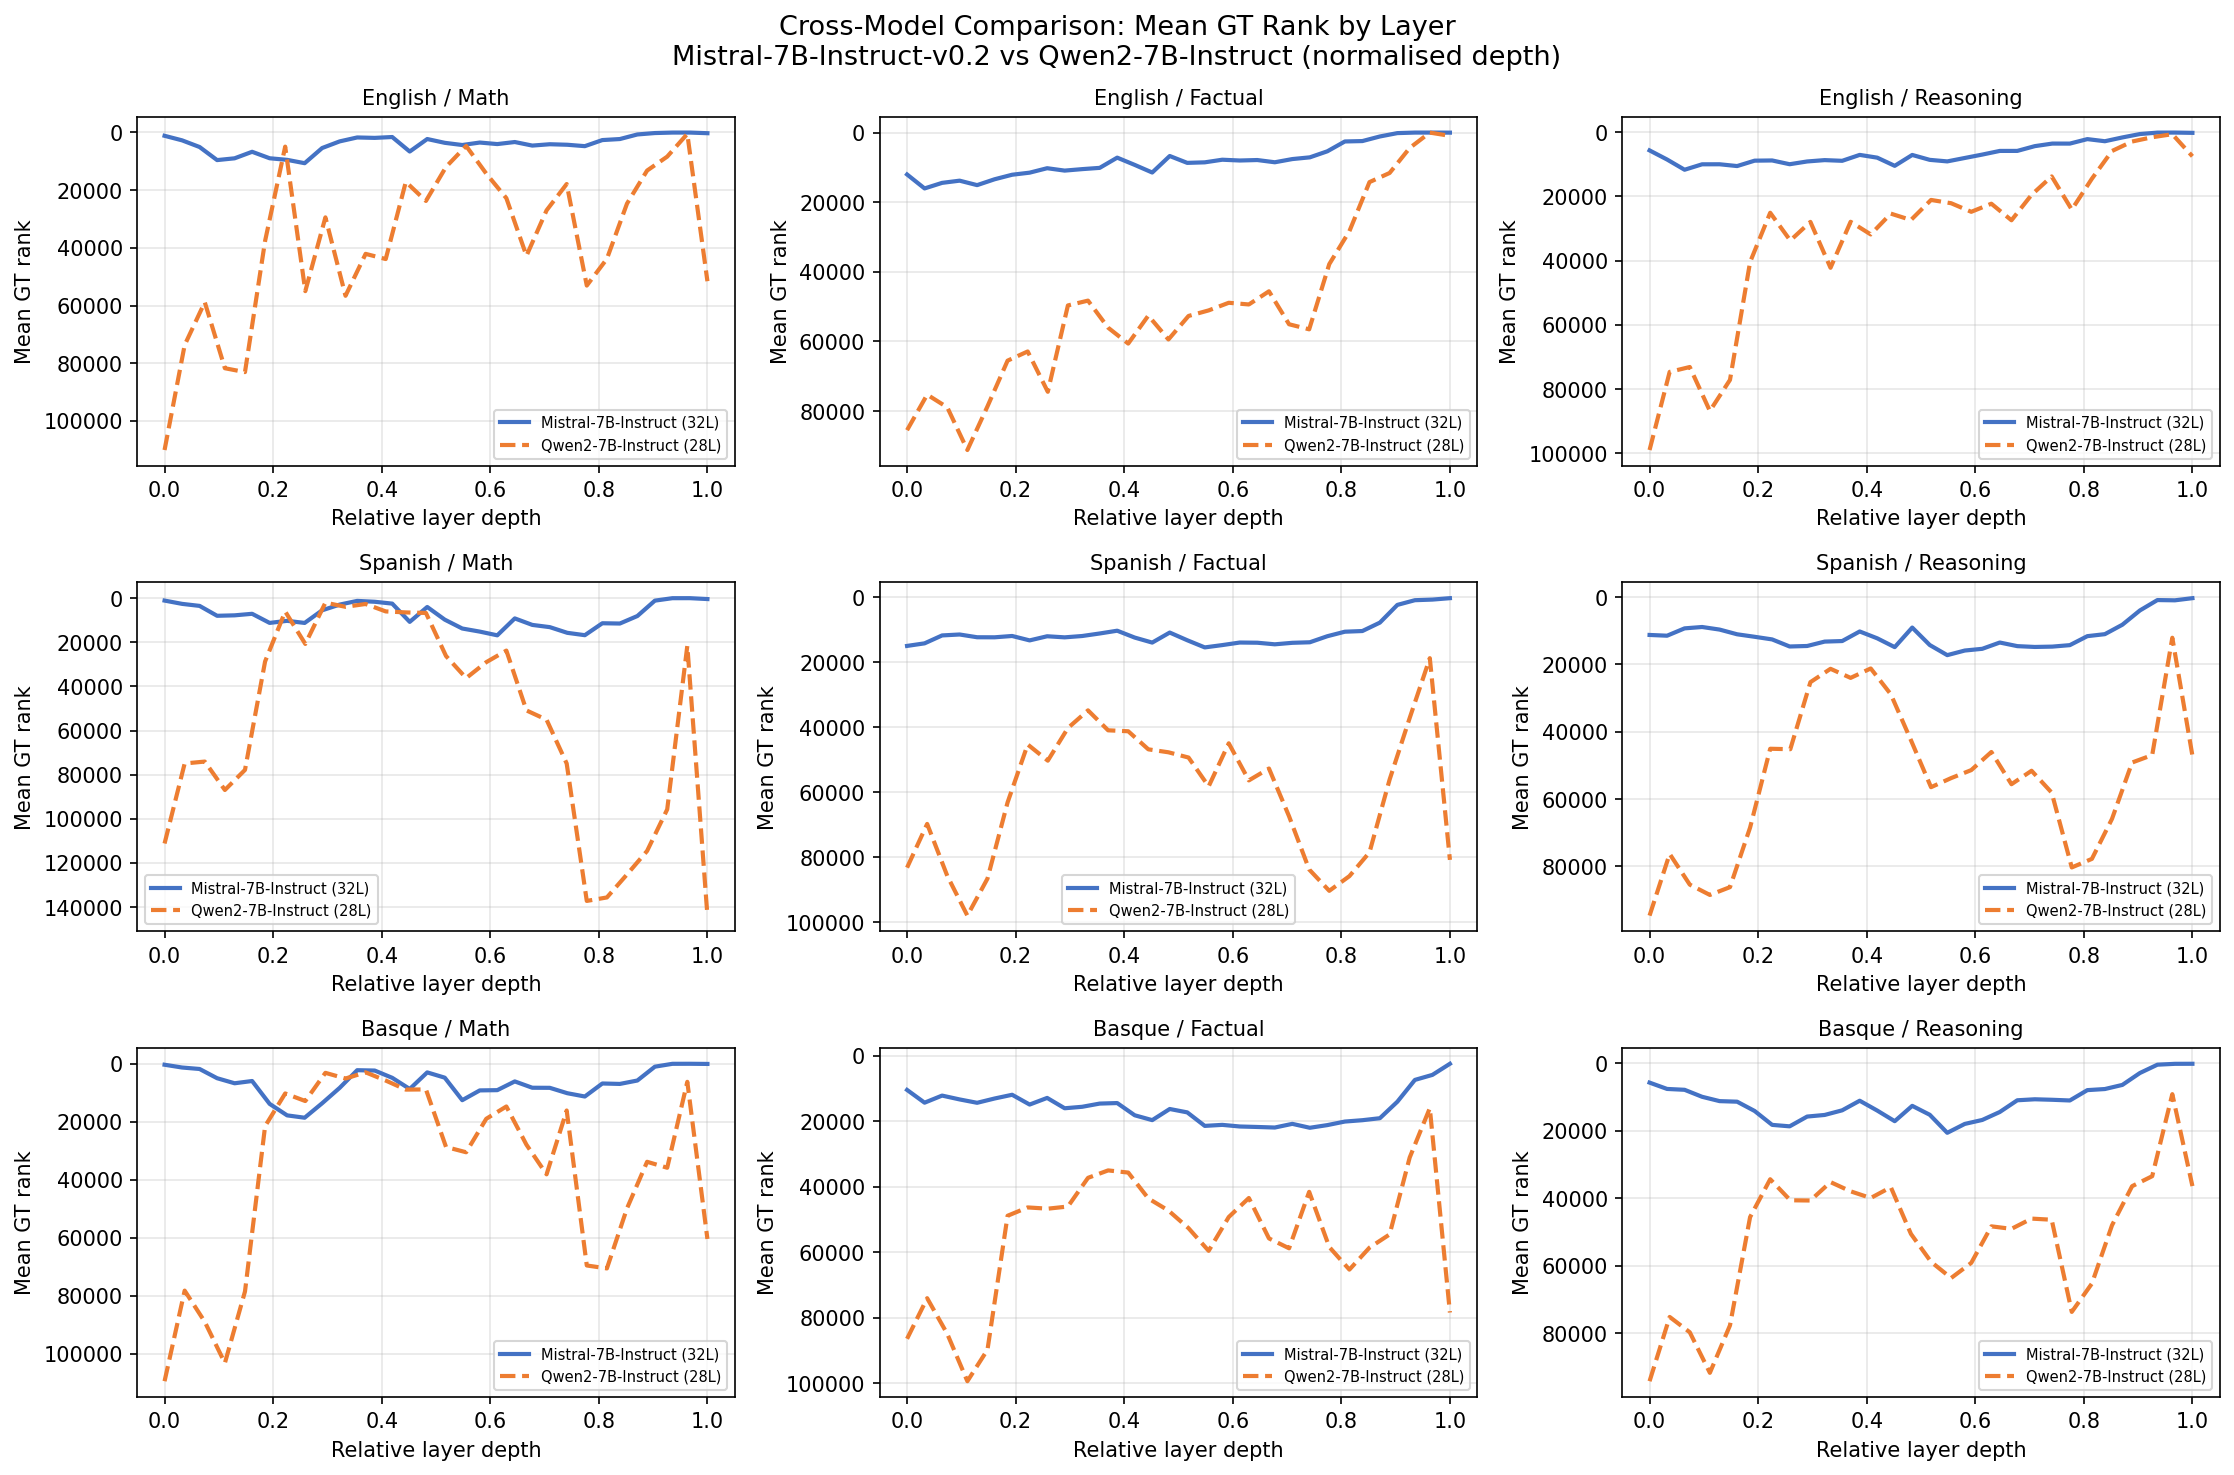
\includegraphics[width=\linewidth]{figures/fig7_cross_model_gt_rank.png}
\caption{GT rank trajectories: Mistral (solid), Qwen2 (dashed). Trajectory shapes comparable; Qwen2's larger vocab inflates absolute ranks.}
\label{fig:cross_model}
\end{figure}

%% ============================================================
\section{Discussion}
%% ============================================================

\paragraph{Black-box accuracy and the Basque collapse.}
Mistral collapses on Basque (8\% overall, 0\% factual) while Qwen2 is far more robust (37\% overall, 65\% Basque math). Factual knowledge is the most vulnerable for low-resource languages; math's numerical answers partially hedge against language-specific gaps. Basque shows a stark discontinuity (e.g., Mistral 60\% $\to$ 8\%; EN--EU factual RSA $\to$ $-$0.049). Below a critical training-data threshold, models may tokenize without meaningfully processing.

\paragraph{Logit lens.}
Math is language-agnostic in early layers: Basque math has \emph{lower} GT rank at L1 (339) than EN/ES ($\sim$1,150) because numerals tokenize identically. Basque factual fails to converge---GT rank 2,440 at L32 vs.\ 26 for English---mirroring 0\% accuracy and showing ``decisive but wrong'' internal predictions. Basque reasoning has the lowest final-layer confidence (53.9\%), consistent with diffuse, incoherent processing. Math is the most language-agnostic across analyses (best early GT ranks, highest EN--EU RSA), as numeric answers are language-invariant.

\paragraph{RSA and implicit translation.}
Math shows the strongest cross-lingual alignment (EN--ES $r = 0.785$ at L32; EN--EU stays positive at 0.389). EN--EU factual RSA collapses to $-$0.049 at L32---structurally random---consistent with Basque factual content being tokenized but not routed through English-style knowledge circuits. EN--ES \emph{reasoning} RSA peaks at L8 ($r = 0.810$) then declines to 0.558 at L32, supporting implicit translation: shared mid-layer representation, then language-specific output. Early layers show moderate Basque alignment (L1 EN--EU factual 0.508) from surface features before language-specific divergence.

\paragraph{Cross-model dissociation.}
Qwen2 achieves better Basque accuracy (37\% vs.\ 8\%) but \emph{lower} EN--ES RSA than Mistral (e.g., reasoning 0.196 vs.\ 0.558). The dissociation suggests different multilingual strategies: Mistral aligns EN--ES strongly but has little usable Basque representation; Qwen2's more uniform multilingual space supports Basque at the cost of weaker EN--ES convergence. Qwen2's larger vocabulary (152K vs.\ 32K) may help Basque tokenization and accuracy without strengthening EN--ES alignment.

\paragraph{Limitations.}
Small benchmark (20 per cell), LLM-as-judge bias risk, two 7B models only; RSA uses last-token only.

%% ============================================================
\section{Conclusion}
%% ============================================================

We presented a joint behavioral and mechanistic evaluation of cross-lingual generalization in two 7B instruction-tuned models, Mistral-7B and Qwen2-7B, over a 180-question benchmark in English, Spanish, and Basque. By combining black-box accuracy with logit lens and Representational Similarity Analysis at every layer, we showed that performance gaps are not merely surface-level but are reflected in the structure of the residual stream.

Our main findings are threefold. First, low-resource language support varies sharply by model and task: Mistral collapses on Basque (8\% overall, 0\% factual) while Qwen2 remains substantially more robust (37\% overall), and factual knowledge is the most vulnerable category. Second, layer-wise probing reveals where this failure occurs: math answers are identified at shallow layers regardless of language (and Basque math can even show better early GT rank than English), whereas Basque factual representations fail to converge by the final layer---the model is ``decisive but wrong.'' Third, RSA provides evidence for implicit translation in reasoning: English--Spanish representational similarity peaks in mid-layers (e.g., $r = 0.81$ at layer 8) then declines at the output, consistent with a shared internal reasoning stage followed by language-specific generation. At the same time, the cross-model comparison shows that better Basque accuracy need not coincide with stronger EN--ES alignment; Mistral and Qwen2 appear to adopt different multilingual representational strategies.

These results suggest that layer-wise RSA and logit lens are practical tools for diagnosing \emph{where} and \emph{how} cross-lingual generalization breaks down, with implications for model selection, data curation, and interpretability in multilingual deployment. Future work should extend the benchmark to more languages and larger models, test whether activation patching (e.g., substituting English or Spanish residual streams into Basque forward passes) can improve Basque accuracy, and analyze correct versus incorrect answer trajectories to see whether successful cross-lingual processing shows earlier or stronger representational alignment.

%% ============================================================
\bibliographystyle{abbrvnat}
\bibliography{references}
%% ============================================================

\end{document}
